\Mat{
   a,b\in \mathbb{R}, \ n\in\mathbb{N}\\
   \forall \ a>0, n>1 \ : \ \exists! \ b>0 \ : \ b^n=a \\
   \text{jele:}\ b=a^{\frac{1}{n}}
}
Továbbá:
\Mat{
   (a^{\frac{1}{n}})^m=(a^m)^\frac{1}{n},
}
így lehet beszélni egyszerűen $a^{\frac{m}{n}}$-ről.

\vspace{1cm} Indoklás. 
Legyen $a>1$ és
\Mat{
   a_{-}=\{ b\ :\ b^n < a \}\\
   a_{+}=\{ b\ :\ b^n > a \}
}
Megfigyelések:
\begin{itemize}
   \item $a_{-}$ és $a_{+}$ nemüresek
   \item bármely $b\in a_{+}$ felső korlátja $a_{-}$
   \item bármely $b\in a_{-}$ alsó korlátja $a_{+}$
\end{itemize}
A valós számok felső/alsó-határ tulajdonsága miatt egyértelműen létezik
$S=\sup a_{-}$ és $I=\inf a_{+}$ és $S\le I.$
\Dnew{}

Ha $S < I$ akkor az ábra segít megtalálni az ellentmondást:
\begin{center}
\frame{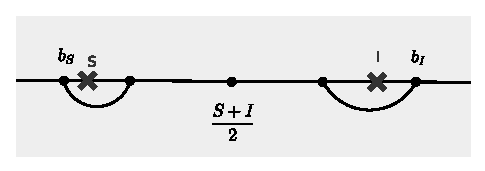
\includegraphics[scale=1.2]{DB/fig/nthroot}}
\end{center}
Tehát $S=I.$ Ezért: $I^n = S^n \le a$ és $I^n\ge a$, vagyis az $S=I$ szám
valóban $a^{\frac{1}{n}}$-ként viselkedik.

Ha $y=\gzjel{a^m}^\frac{1}{n}$ és $z=\gzjel{a^\frac{1}{n}}^{m}$, akkor
\Mat{
   y^n=a^m \\
   z^n=\gzjel{a^\frac{1}{n}}^{mn}=\gzjel{\gzjel{a^\frac{1}{n}}^n}^{m}=a^m,
}
ezért mindkettő az $a^m$ szám $n$-ik gyöke, ami egyértelmű $\implies y=z.$
